\subsection{Parameter Tuning}

using datasets: all mixed 5 + 5

\subsubsection{Raw Performance}

\begin{figure}[H]
\centering
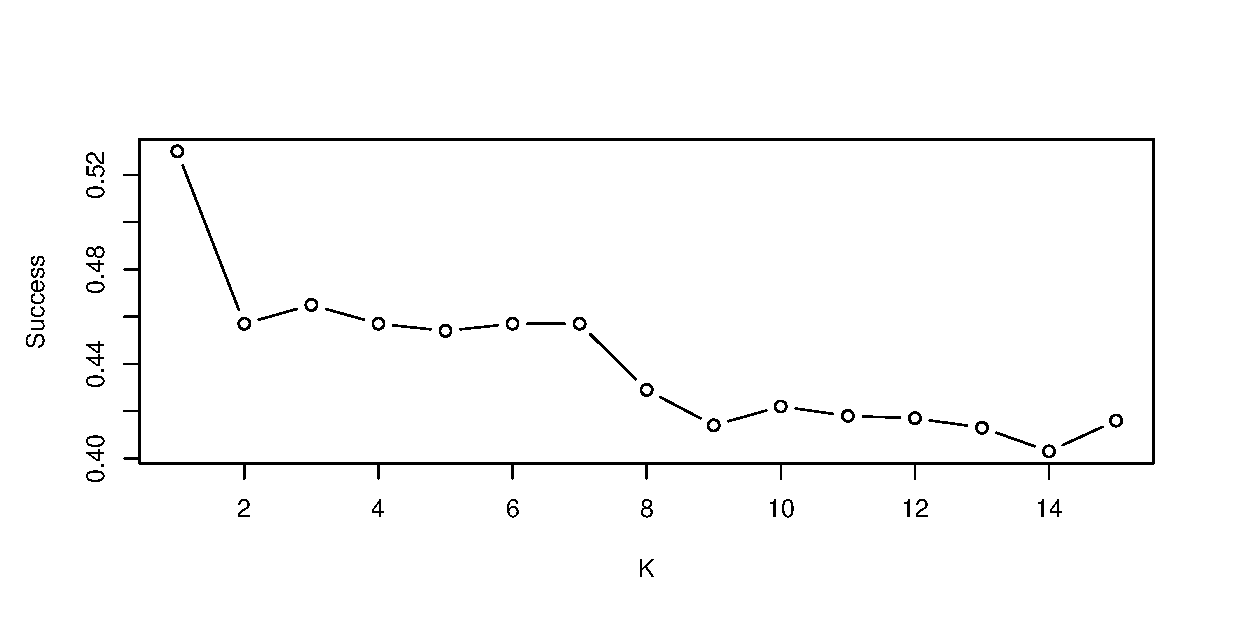
\includegraphics[width = 0.9 \textwidth]{graphics/knn_raw_success}
\caption{Success for K-NN with no preprocessing used.}
\end{figure}


\subsubsection{Smoothing}

\begin{figure}[H]
\centering
\missingfigure{cont. sigma vs size}
\end{figure}


\subsubsection{Principle Component Analysis}

\begin{figure}[H]
\centering
\missingfigure{sigma/size vs PC or success vs PC if best smoothing distinct}
\end{figure}


\subsubsection{Z-Score}

\begin{figure}[H]
\centering
\missingfigure{success for raw, pre zs, post zs and both}
\end{figure}


\subsubsection{Performance}

\begin{figure}[H]
\centering
\missingfigure{Confusion with all the best parameters for the full dataset easy problem}
\end{figure}

\begin{figure}[H]
\centering
\missingfigure{Confusion with all the best parameters for the full dataset difficult problem}
\end{figure}




\subsubsection{PCA}

Calculating with less data will result in a faster computation time.
However, choosing too few PC results too few features left to compare.
To see how the performance and the timing scales both are shown in figure \ref{fig:pca_timing_lukas} and \ref{fig:pca_timing_nikolaj}. K was chosen to be 10.
In figure \ref{fig:pca_timing_lukas} the performance seems to be the same regardless of how many PC is chosen. As long as there are more than 60 the performance will be the same.
On the test done on Group member 1 the performance is worse which means the digits are less uniform. 
Here the success rate has a peak with a low set of attributes so there must be some confusion that gets sorted out. 
Both test were run with 100 DPI. The percentage of successful predictions is also measured with the same data.
The timing was measured on the same computer so the difference should not be very large. 

\begin{figure}[H]
\centering
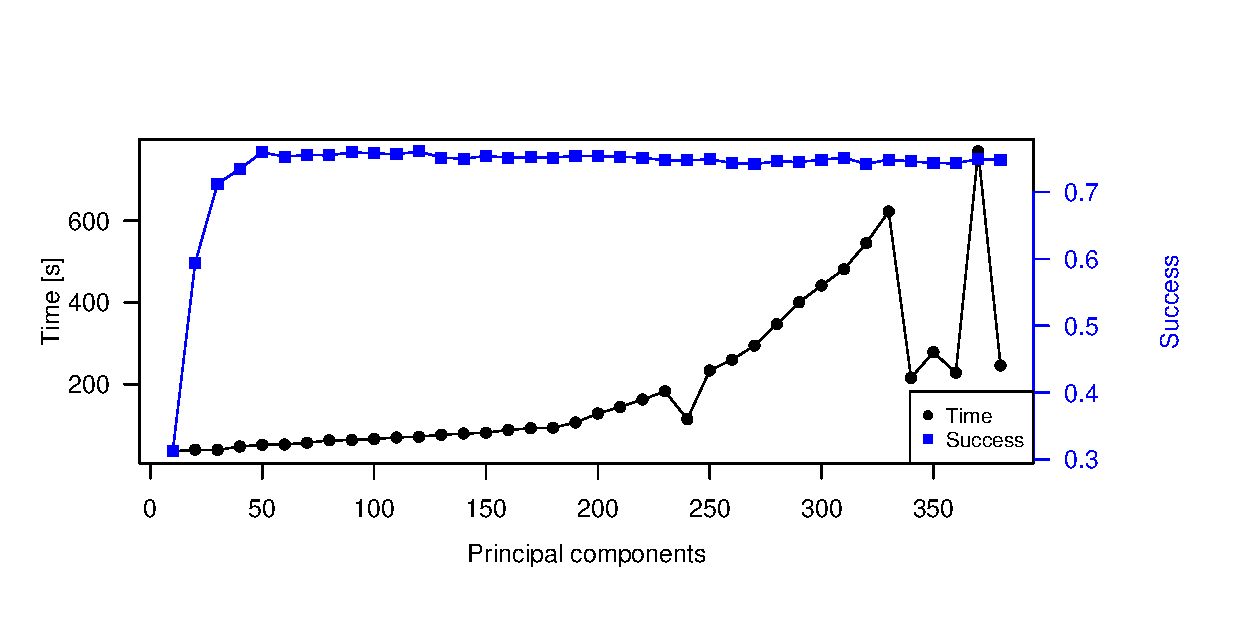
\includegraphics[width =0.8 \textwidth]{graphics/pca_timing}
\caption[Timing of PCA]{Timing of running the PCA with different principle components. 
The data was run on Group 3 member 2's data. 
}
\label{fig:pca_timing_lukas}
\end{figure}
\begin{figure}[H]
\centering
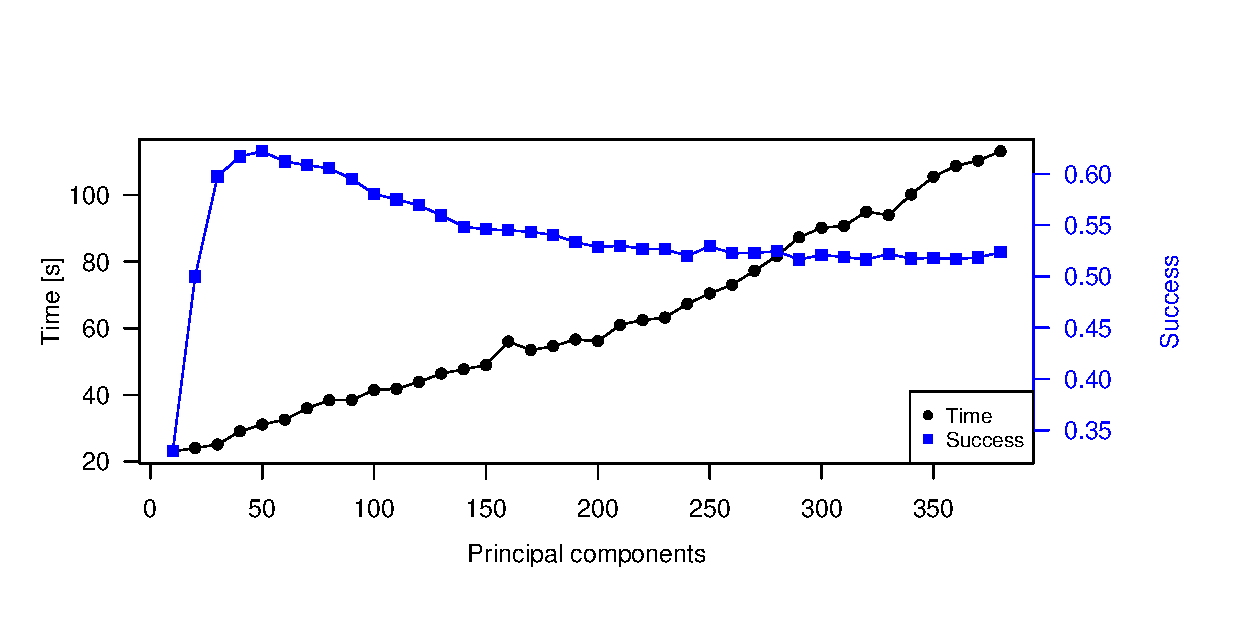
\includegraphics[width =0.8 \textwidth]{graphics/pca_timing_nikolaj}
\caption[Timing of PCA]{Timing of running the PCA with different principle components. 
The data was run on Group 3 member 1's data}
\label{fig:pca_timing_nikolaj}
\end{figure}

To get a closer look at how the PCA performs the data from G3M2 was tested against the rest of the class. 
The K was chosen to be 10. 
The data is shown in figure \ref{fig:pca_success}.
The performance is getting worse as more features are considered.
